\documentclass[12pt]{article}

\usepackage{fullpage}
\usepackage{graphicx, rotating, booktabs} 
\usepackage{times} 
\usepackage{natbib} 
\usepackage{indentfirst} 
\usepackage{setspace}
\usepackage{grffile} 
\usepackage{hyperref}
\usepackage{adjustbox}
\usepackage{amsmath}
\usepackage{siunitx}
\usepackage{multirow}
\setcitestyle{aysep{}}


\singlespace
\title{\textbf{Elite Cues and Public Attitudes Towards Military Alliances}}
\author{Joshua Alley \\
Postdoctoral Research Associate \\
University of Virginia.\thanks{Thanks to Erik Lin-Greenberg, Philip Potter, Justin Schon and Todd Sechser, as well as participants in the Democratic Statecraft Lab Research incubator, the Lansing B. Lee/Bankard Seminar in Global Politics, 2020 Annual Meeting of the Peace Science Society and 2021 Meeting of the International Studies Association for helpful comments. 
This project was reviewed by the University of Virginia IRB (Protocol 3866) and preregistration files for this study are hosted in an OSF repository at https://osf.io/g28zs.} \\
jkalley@virginia.edu
}
\date{}

\bibliographystyle{apsr}

\begin{document}

\maketitle 

\doublespace 

\begin{abstract}
Do elite cues have extensive, conditional or minimal influence on public support for military alliances in the United States? 
In this note, I assess the boundaries of elite leadership on public opinion towards alliances by examining whether partisanship and foreign policy dispositions modify individual responses to elite cues.
I argue that if co-partisan elite cues change public attitudes regardless of baseline alliance dispositions from isolationism and militant assertiveness, elites exert extensive influence. 
Using two conjoint survey experiments to examine public attitudes towards forming and maintaining international alliances, I find that elites can lead most of the electorate, but some individuals hold rigid alliance attitudes. 
These fixed attitudes have a partisan asymmetry, as staunch alliance supporters in the Democratic party and consistent alliance skeptics in the Republican party both discount elite cues.  
Therefore, elites can lead most public opinion towards military alliances, but strong individual concerns occasionally constrain their influence.  
\end{abstract}


\newpage 


\section{Introduction}


% lay out the question
Do elites lead U.S. public opinion towards military alliances, and if so, who follows their cues?
Looking at observational data, the relationship between elite cues and public alliance attitudes is unclear.
For example, many observers feared that Donald Trump would undermine domestic support for alliances, yet U.S. public approval of alliances like NATO increased in most years of the Trump administration and remained steady even among Republicans through 2019 \citep{PewNATO2020}.


Elite cues could exercise extensive, conditional or minimal influence on public alliance attitudes. 
Extensive elite leadership of public opinion is possible given limited public information and interest in foreign policy \citep{Canes-Wrone2006, BaumPotter2008, Druckman2014}.
There is also evidence that leaders often conform their rhetoric to public attitudes, however, so elites might have minimal influence  \citep{Barberaetal2019, HagerHilbig2020}.
Even when the public pays little attention to international affairs, their opinions have consistency and structure \citep{Holsti1992, PageShapiro1992}.
Individual foreign policy dispositions like isolationism and militant assertiveness \citep{Herrmannetal1999, KertzerZeitzoff2017} could establish alliance attitudes for elite cues to match.\footnote{This article considers the leading or following question for Trump and NATO: \url{https://fivethirtyeight.com/features/is-trump-fueling-republicans-concerns-about-nato-or-echoing-them/}}
Last, perhaps elites exert conditional influence, as some of the public follows their cues and others do not. 
Some individuals may hold more rigid alliance opinions than others.


The extent of elite leadership shapes the role and relevance of public opinion in alliance politics.
If elites cues lead public opinion, then public attitudes are unlikely to constrain elite alliance decisions.
But if individual attitudes are unresponsive or conditionally responsive to elite cues, then public opposition could undermine forming new alliances or withdrawing from existing treaties. 
Thus, elite influence on public opinion is crucial to understanding the domestic politics of U.S. alliance formation and maintenance.  


Despite the importance of elite-public interactions in alliance politics, we do not know how partisan and other elite cues affect public attitudes towards alliance commitments. 
Most evidence comes from opinion polls measuring public sentiment towards alliances like the North Atlantic Treaty Organization (NATO).
These polls provide useful data, but they cannot establish a causal connection between elite cues and public attitudes.


% contribution
To delineate the boundaries of elite influence on U.S. alliance attitudes, I assess whether foreign policy dispositions and partisanship change individual responses to partisan elite cues.
How co-partisan elite cues impact individuals with different predispositions towards alliances from isolationism and militant assertiveness shows who elites lead because partisanship and foreign policy dispositions set initial alliance attitudes. 
Isolationism increases skepticism of alliances, while militant assertiveness makes individuals more likely to back alliance participation. 
If co-partisan elite cues sway public opinion regardless of initial dispositions from hawkishness and isolationism, elites exert extensive influence. 
But if co-partisan elite cues impact a minute or limited portion of the electorate, their influence is minimal or conditional.


% Assess w/ a survey experiment
I use two conjoint survey experiments to provide causal evidence on elite leadership of public opinion towards alliances.
This approach allows me to randomize many alliance characteristics and elite cues \citep{Hainmuelleretal2014}.
Unlike in observational data, an experiment that randomly assigns elite cues can leverage information on foreign policy dispositions within parties to distinguish who follows elite cues. 
The first experiment scrutinizes attitudes towards alliance formation, while the second addresses alliance maintenance. 


% findings: 
In two nationally representative samples, I find extensive elite leadership with two important limits.
While most individuals follow co-partisan elite cues regardless of their foreign policy dispositions, a few do not.
The strongest Democrat alliance supporters have rigid alliance attitudes, as do staunch Republican alliance skeptics. 
Partisanship and foreign policy dispositions also set the level to which elite cues move alliance attitudes.
Elite cues thus exert broad influence, but their impact depends on partisanship, militant assertiveness and isolationism.


The partisan divide in rigid alliance attitudes is especially noteworthy.
Hawkish and isolationist Democrats are robust alliance supporters.\footnote{Roughly 25\% of Democrats in both experiments express a mix of isolationism and and militant assertiveness by agreeing with staying home instead of addressing international concerns while also expressing willingness to use force in international affairs.}
Dovish and isolationist Republicans are committed alliance skeptics.\footnote{Approximately 8\% of Republicans in both samples hold isolationist and dovish views, as most Republicans score highly on militant assertiveness.} 
Therefore, Republicans can lead the most likely alliance supporters in their party and Democrats can lead relative alliance skeptics. 
If elected leaders follow the strongest alliance attitudes in their party, they will polarize everyone else. 


% differences between formation and mainteance
%Furthermore, public support for alliance maintenance is higher and less responsive to elite cues than support for alliance formation.
%Even with opposition from one set of co-partisan elites, upholding existing alliances almost always retains majority support. 
%In alliance formation, elite cues determine whether a new treaty has majority or minority support. 
%Therefore, elites have more influence over forming new alliances than changing existing commitments. 


% Importance part 1: public opinion undergirds alliance com in democ
In addition to providing new insight into debates over elite leadership of public opinion, there are two reasons that understanding U.S. public opinion towards alliances is worthwhile. 
For one, public opinion is central to debates over whether democracies make more reliable commitments than other states.\footnote{Public opinion is important, but it is not deterministic. \citet{Kreps2010} notes that public disapproval may not hinder coalition warfare, especially when elite consensus favors fighting.} 
If public opinion towards alliances is indifferent to elite cues, stable attitudes and reliable commitments are more likely \citep{Gaubatz1996}.
If elite cues drive public opinion, then public attitudes may shift quickly, leading to cycles that hinder democratic reliability \citep{GartzkeGleditsch2004}.


% importance part 2: practical relevance- US role in world. 
%The impact of elite cues on alliance attitudes also speaks to the consequences of a prominent scholarly and policy debate. 
%Two competing visions of U.S. foreign policy argue about alliances. 
%One perspective believes that the United States should reduce its alliance commitments to pursue a restrained grand strategy \citep{Preble2009, Posen2014}.
%The other argues that continued deep engagement through alliances is the best way to promote U.S. security and prosperity \citep{Brooksetal2013, BrandsFeaver2017}. 
%If elite cues have extensive influence, leaders will face limited public constraints on implementing their grand strategic vision. 


% importance part 3: WHY support international cooperation, not just consequences of international institutions
This study also fills a gap in international institutions scholarship. 
Scholars are more likely to study how international institutions affect public attitudes (e.g. \citep{KayaWalker2014, Greenhill2020}), than scrutinize the sources of public attitudes towards international institutions themselves. 
Other studies use observational survey data to examine public opinion towards international cooperation in multilateral financial institutions \citep{Edwards2009} or the United Nations \citep{Torgler2008, DellmuthTallberg2015}. 
The result is limited causal evidence on individual alliance attitudes.
In one study of public opinion and military alliances, \citet{TomzWeeks2021} address a different question by showing that the presence of an alliance increases public support for foreign military intervention. 
\citet{Chuetal2021} explore how values and interest based elite cues shape public attitudes towards alliance maintenance. 
I build on these works with more general experiments on alliance formation and maintenance that clarify the reach of partisan and other elite cues while accounting for many alliance characteristics. 


% Implications
The finding that elite cues have substantial influence on public alliance attitudes while some individuals hold rigid opinions has important implications for U.S. alliance politics. 
Although elite cues affect public support for U.S. alliances, they do not reach the whole electorate.
Also, one set of elites cannot produce majority opposition to existing treaties by themselves, because alliance maintenance commands substantial support. 
Public backing for new alliance commitments is more responsive to elite cues. 
Therefore, whether political elites follow the contradictory fixed attitudes in the two major parties will shape domestic support for U.S. alliances, especially new commitments.

% Try it w/o the plan of paper for flow. 


\section{Elite Leadership and Alliance Attitudes}


Public opinion molds democratic foreign policy and alliance politics in several ways.
First, it affects elite military intervention decisions \citep{Tomzetal2020, LinGreenberg2021}. 
In democracies, anticipation of paying public audience costs for alliance treaty violation encourages limited promises of military support \citep{Chibaetal2015, FjelstulReiter2019}. 
Moreover, public attitudes are central to disputes about the reliability of democratic commitments \citep{Gaubatz1996, GartzkeGleditsch2004}. 
As a result, policymakers heed public support for alliances \citep{Sayle2019}. 


% NATO example to bring out the puzzle
%In addition to its importance, there is meaningful variation in pubic opinion towards military alliances. 
%\autoref{fig:nato-op-time} plots the percentage of respondents supporting NATO in 59 surveys from 1974 to 2020.\footnote{These surveys ask respondents to assess NATO in many ways. I consider favorable opinions, feeling thermometer ratings of 50 or higher, and support for increasing or maintaining U.S. commitment as indicators of support for NATO.} 
%Most surveys show majority support for NATO, but average support fell after 2000.  
%
%
%\begin{figure}
%	\centering
%		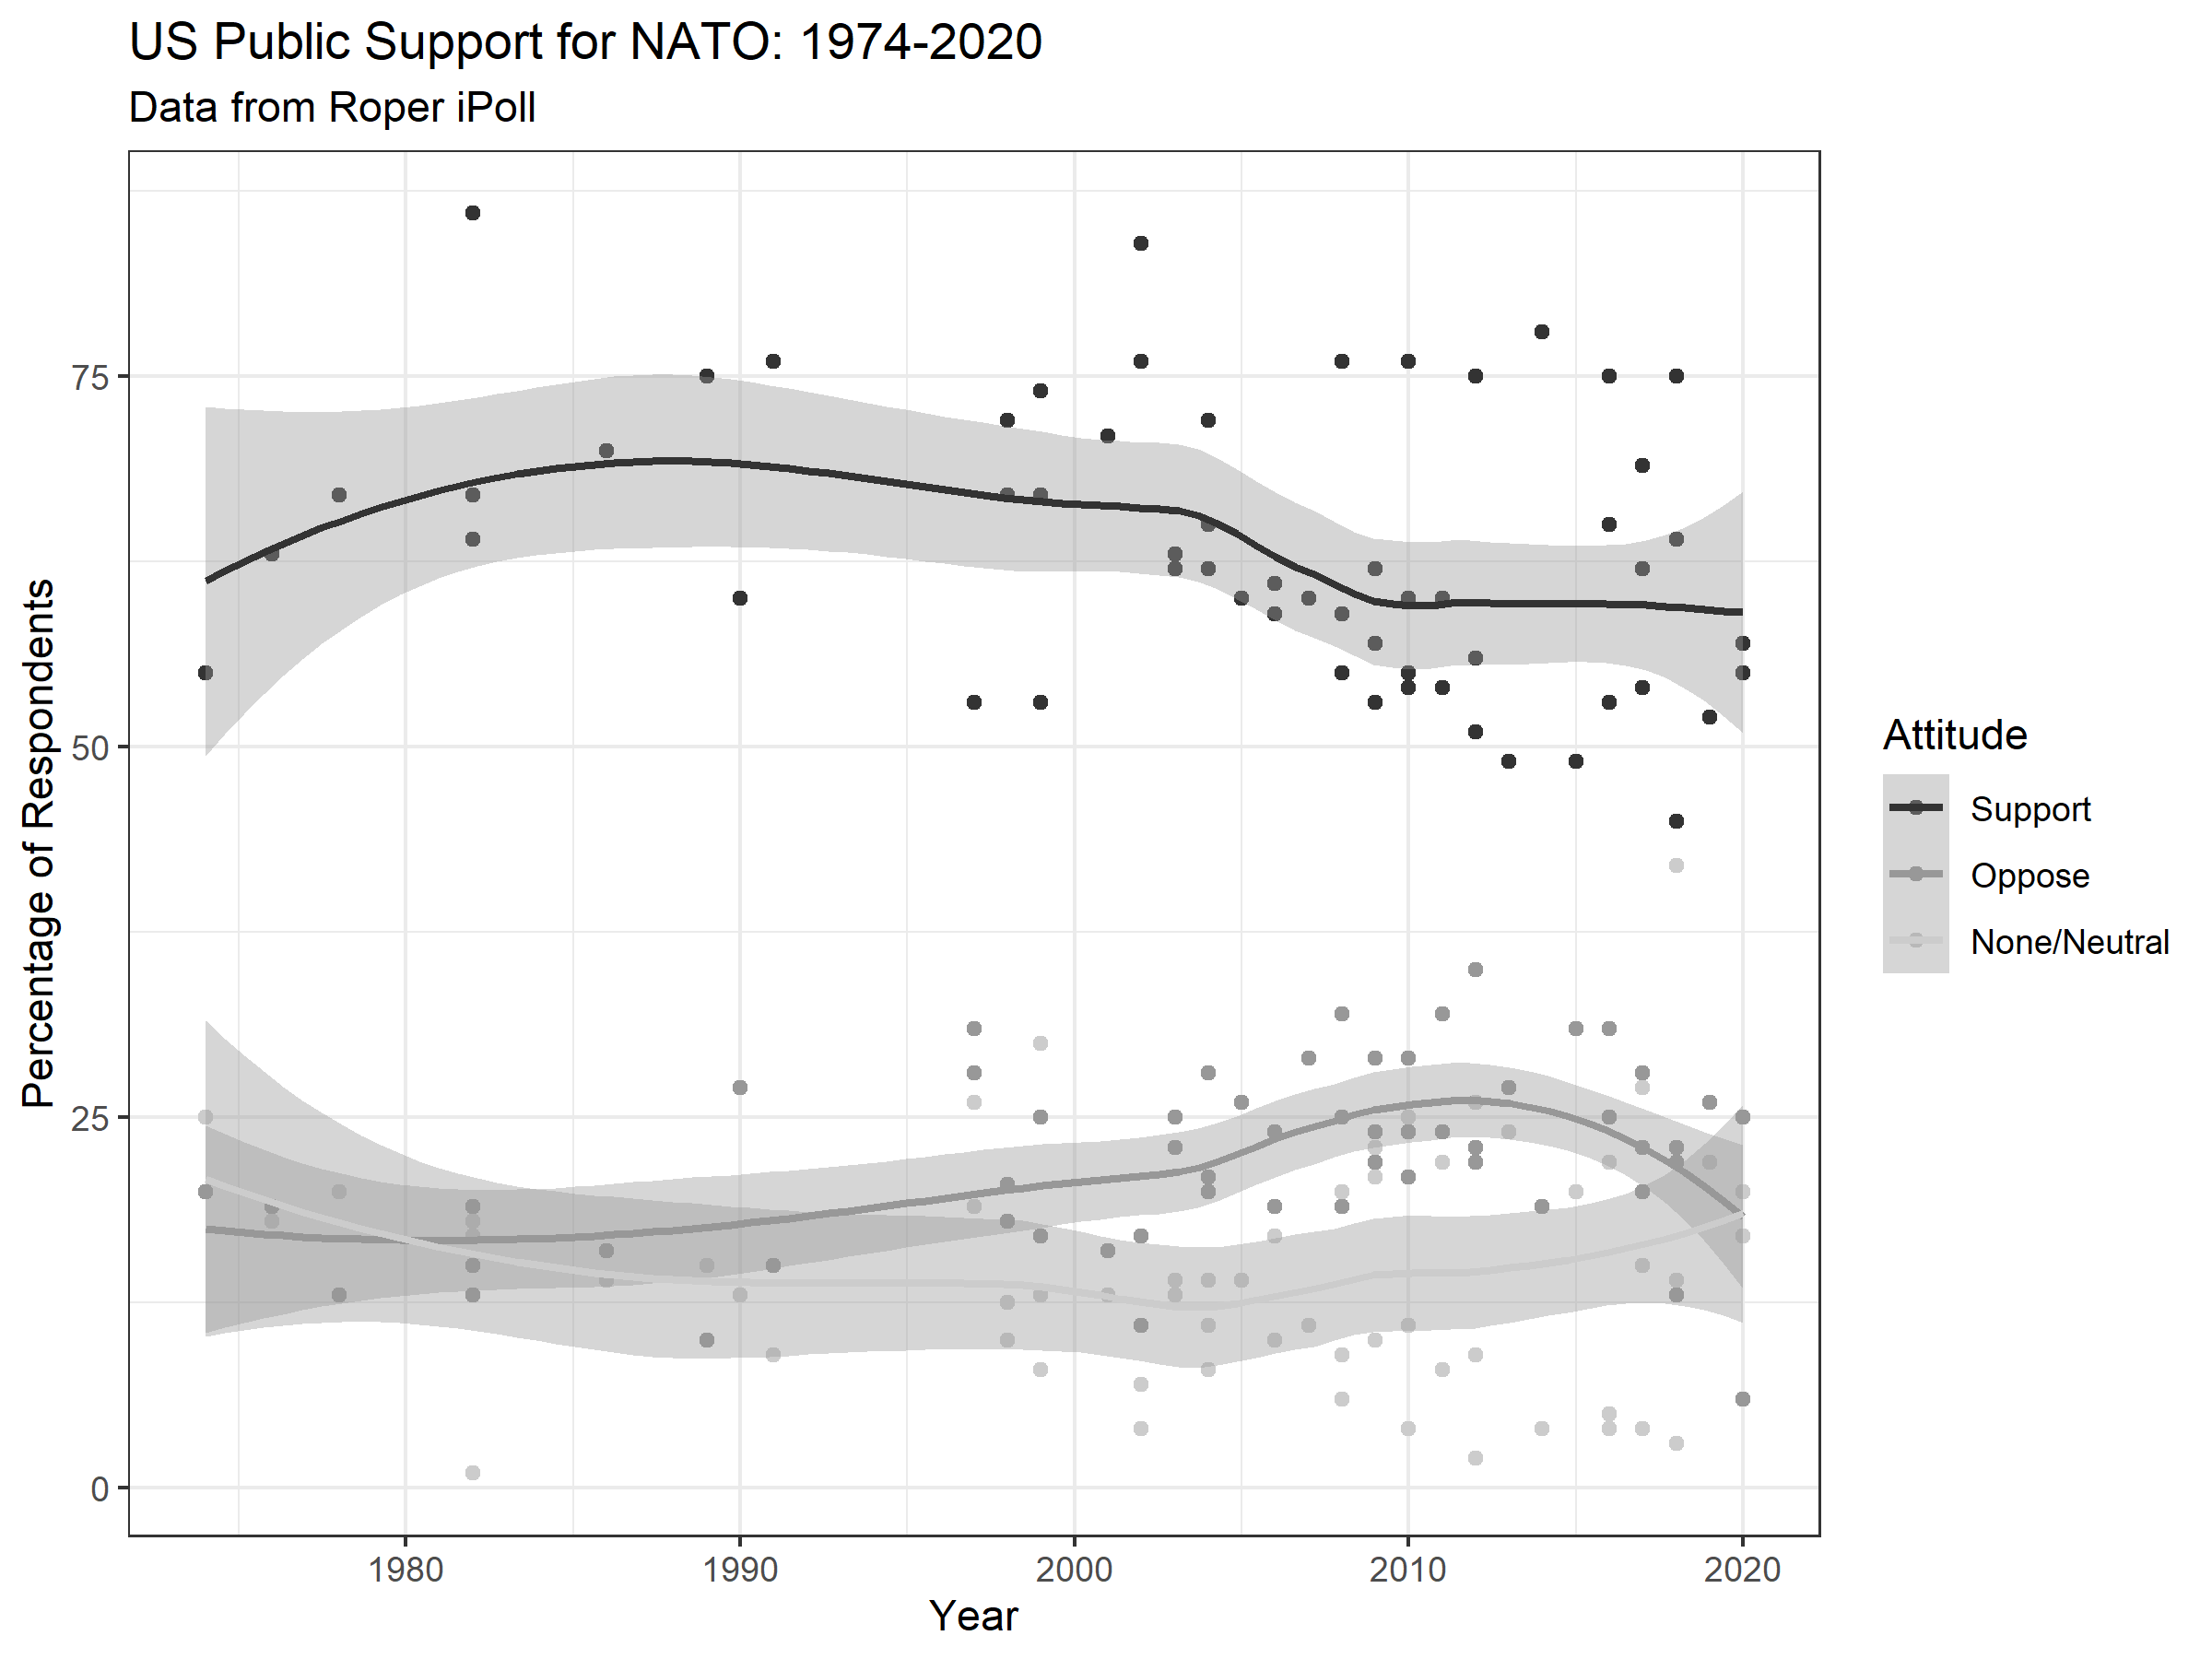
\includegraphics[width=0.95\textwidth]{../figures/nato-op-time.png}
%	\caption{US public support for NATO from 1974 to 2020. Each point marks a unique poll, and colors differentiate the percentages of respondents that expressed support, opposition or neutral/no opinion of NATO. Loess lines estimate the average support for each group in every year. Topline data from the Roper Center's iPoll database.}
%	\label{fig:nato-op-time}
%\end{figure}


Even as policymakers track alliance attitudes, observed opinions are subject to a longstanding puzzle in public opinion on foreign policy.
When we observe elite and public support for alliances, it is unclear if public attitudes follow elite cues, if only some of the public responds to elite cues or if elite cues reflect public opinion. 
All three perspectives offer plausible models. 


Whether elites lead or follow public opinion is unclear.
Some suggest that elites are more likely to lead public opinion. 
\citet{Canes-Wrone2006} finds that U.S. Presidents rarely follow public preferences they disagree with and have ample freedom to lead foreign policy attitudes. 
\citet{JacobsShapiro2000} argue that elites track public opinion to manipulate it, not conform to it. 
\citet{Kreps2010} notes that public disapproval did not constrain participation in NATO's International Security Assistance Force in Afghanistan. 
Moreover, foreign policy is a secondary concern for many voters, so elite foreign policy views and rhetoric can diverge from public attitudes with few political repercussions \citep{BusbyMonten2012}. 


Other findings suggest that elites conform their rhetoric and policy stances to public opinion. 
\citet{Barberaetal2019} use social media data to show that legislators are more likely to follow than lead public opinion, including on some foreign policy issues. 
\citet{HagerHilbig2020} find that exposure to public opinion research moves speech and policy positions by German politicians closer to majority opinion. 
\citet{Haesebrouck2019} uncovers little evidence that European elites led public support for military interventions in Libya and the Islamic State. 
\citet{Bechteletal2015} find that elite cues and frames led Swiss individuals, especially those with low knowledge, to reinforce their prior immigration attitudes. 
Even military elites who have no electoral concerns shape their policy recommendations in response to public opinion \citep{LinGreenberg2021}. 


Conditional elite influence is also possible. 
\citet{PageShapiro1992} note that public opinion is broadly consistent and rational, and changes in predictable ways in response to information from multiple sources, including elite cues. 
\citet{GuisingerSaunders2017} claim that for issues with low partisan polarization, information effects dominate public opinion, though elite cues matter more for polarized issues like cap and trade schemes.\footnote{\citet{GuisingerSaunders2017} map the boundaries of elite influence across issues. In the following, I focus on who responds to elite cues in alliance politics.}
Democrats express higher support for alliances like NATO than Republicans \citep{PewNATO2020}, but the partisan gap in alliance attitudes is smaller than polarized issues like the Iran nuclear program but larger than more technical issues such as the International Criminal Court treaty \citet{GuisingerSaunders2017}. 


%Elites could therefore exert extensive, minimal or conditional influence on alliance attitudes. 
%Limited public information about alliances could encourage broad elite influence \citep{Druckman2001}.
%Public opinion towards alliances might instead depend on individual concerns that limit minimize elite influence.
%Foreign policy dispositions are especially important, as these intuitions about international affairs provide consistent heuristics even with limited information \citep{Herrmannetal2009, KertzerZeitzoff2017}.
%Conditional elite influence is also possible, as some alliance attitudes may be more plastic than others.  


Understanding alliance attitudes thus addresses a fundamental debate about public opinion on foreign policy. 
In the following, I examine the extent of elite cues' influence on public opinion towards alliances.\footnote{I do not fully address if elite cues follow public opinion, as I do not show what drives elite cues. Rather, I assess a crucial component of elite leadership that cannot be inferred from observational data.}
To do so, I assess whether all, some, or little of the electorate responds to elite cues based on their predispositions towards alliances.
The remainder of this argument explains how partisanship and foreign policy dispositions determine who might hold rigid alliance attitudes and which responses to elite cues reflect extensive elite leadership. 
I first outline the general process of elite cue leadership. 


\subsection{Elite Cues} 
% Framing/elite leading


Under a simple elite cues model the public follows trusted elites in forming their opinion, so elite portrayals of alliances bolster or undermine public support.
Public opinion towards alliances thus permeates down from the top and is endogenous to elite views \citep{Druckman2014}.
There is substantial evidence that elites influence public foreign policy attitudes \citep{BaumPotter2008}. 
The media often convey elite cues and frames.
Social media may further amplify elite influence \citep{BaumPotter2019}.   


Elite support or opposition could shape alliance attitudes because individuals rely on trusted elites in an issue environment with little alternative information. 
Information shortcomings make individuals more responsive to elite framing and cues \citep{Druckman2001, Peterson2017} and the public lacks foreign policy information \citep{BaumPotter2008}.
Furthermore, alliance politics is a less salient foreign policy issue than international conflict, which is the most common subject in studies of foreign policy opinions. 


% cue-giver matters 
Multiple elites can give public alliance cues.
Elected officials, diplomats and military leaders all participate in alliance politics.
The public visibility and influence of elected leaders is well-established.  
Cues from military leaders can shape public opinion about the use of force \citep{Golbyetal2018}, so military endorsements may also move alliance attitudes. 
Diplomatic elites are high profile experts. 
Public perceptions that military leaders and diplomats are well-informed about alliances will likely increase their influence. 


% highlight partisanship
In an elite cues model, support for alliances by trusted elites should increase individual support for alliances, and elite opposition will reduce support.   
Partisanship helps elites establish trust and makes co-partisan elite cues more influential \citep{Druckmanetal2013}.
Under partisan polarization, individuals distrust and discount messages from out-partisan elites.
As a result, bipartisan or unified elite cues encourage robust public support \citep{Berinsky2007}.


% transition paragraph: scope of influence
Elite cues are a straightforward and compelling explanation of alliance attitudes.
Even information about alliance characteristics like allied democracy or military spending likely reaches the public through elite rhetoric. 
This makes extensive elite influence on alliance attitudes plausible. 
When they receive elite messages, individuals also hold prior attachments, intuitions and beliefs, however.
Individual foreign policy dispositions and partisanship could set initial alliance dispositions and modify whether alliance attitudes are rigid or plastic under elite cues. 


\subsection{Foreign Policy Dispositions and Partisanship}


% Overview para
Foreign policy dispositions and partisanship shape individual perceptions of international politics. 
These individual concerns have two consequences for alliance attitudes. 
First, they establish individuals' baseline alliance support, or willingness to back alliances in general.\footnote{Another way to think of baseline support is an individual disposition to support an average or typical alliance.} 
Second, individual concerns might change individual responses to elite cues. 
Individuals could hold prior attachments so tightly that elite cues have minimal influence, or alliance predispositions could make some individuals responsive and others unresponsive, resulting in conditional elite influence.


% foreign policy disposition
Foreign policy dispositions are intuitions about international politics \citep{KertzerTingley2018}. 
Such principles shape how people respond to decisions such as backing down from military intervention threats \citep{KertzerBrutger2016}. 
Militant assertiveness and internationalism are two key foreign policy dispositions for alliance attitudes \citep{Herrmannetal1999}.\footnote{While internationalism and militant assertiveness are continuous concepts, I discuss them in categorical terms to maintain consistency with the experimental results, which require categorical foreign policy disposition indicators.}
These dispositions set baseline inclinations towards alliances before individuals receive elite cues.\footnote{To give a related example from a different domain, \citet{KertzerBrutger2016} leverage foreign policy dispositions to decompose audience costs into belligerence and consistency costs.}
Whether and how individuals respond to elite cues given their prior dispositions provides insight into elite influence. 


% internationalists more likely
% Define internationalism  
Internationalism is an inclination to engage with other countries and contribute to international endeavors. 
Internationalists support U.S. involvement in foreign affairs and are more likely to favor alliance commitments. 
Conversely, isolationists are skeptical of international institutions and cooperation, dislike foreign involvement and prioritize domestic affairs \citep{Kertzer2013}. 
As a result, historic isolationist opposition to alliances is well established. 
Isolationist senators like Robert Taft were the core of U.S. opposition to ratifying NATO \citep{Kaplan2007}.
A U.S. tradition of discomfort with ``entangling alliances'' only broke after World War II \citep{Kupchan2020}.


% militant assertiveness 
Militant assertiveness reflects individual approbation of using force to address international problems \citep{Herrmannetal1999}. 
Dovish individuals are low on militant assertiveness and prefer nonviolent policies.
Hawkish individuals are more willing to employ force.
Although alliances are cooperative institutions that attempt to deter conflict, they also aggregate military capability and obligate members to fight.
General skepticism of using military force should make doves less likely to support military alliances that commit their country to fight.  
European pacifists are among the most consistent NATO opponents, for example \citep{Thies2015}.


Unlike doves, I expect that hawks value capability aggregation through alliances and are more willing to hazard foreign wars. 
Committing to fight for allies is less problematic to hawkish individuals. 
In-group loyalty is a key source of militant assertiveness \citep{Kertzeretal2014} and could increase support for alliance participation by emphasizing group cohesion in the face of external pressures.


% introduce/transition partisanship
Along with internationalism and militant assertiveness, partisanship has an important role in alliance attitudes. 
Party identification connects elite cues and individual concerns by determining which elite cues individuals trust.
Moreover, partisanship is correlated with militant assertiveness and internationalism. 
Conservatives in the United States have a longstanding history of isolationism \citep{Kupchan2020}.
Republicans are more hawkish than Democrats as well \citep{Gries2014}. 


% limits 
Understanding alliance attitudes thus requires careful attention to elite cues, partisanship and foreign policy dispositions. 
Although elites are likely influential, the extent of elite influence is unclear because partisanship changes individual perceptions of elite cues and is correlated with foreign policy dispositions that could shape individual alliance attitudes. 
Perhaps Republican leaders' opposition to alliances does not decrease Republican support for alliances, it reflects isolationism in the Republican party, for instance. 
Hawkish or isolationist individuals might also discount elite cues and rely on their disposition towards alliances. 



\subsection{Assessing the Boundaries of Elite Influence}


% how distinguished
To assess elite leadership, I examine how partisan elite cues impact Democrats and Republicans with different predispositions towards alliances.
Partisanship, militant assertiveness and isolationism create distinct individual inclinations to back or oppose alliance participation. 
These inclinations set baseline alliance attitudes. 
How elite cues move attitudes relative to baseline opinions then shows who elites lead. 
If co-partisan elite cues impact most of the electorate regardless of foreign policy dispositions, elites exert extensive influence on alliance attitudes. 
If co-partisan elite cues only affect some attitudes, elite influence is conditional. 
Minimal elite influence means few individuals respond to elite cues. 


% no a priori about different combinations
I expect that internationalism and hawkishness increase baseline alliance support.
Individuals may be isolationist and hawkish, internationalist and hawkish, isolationist and dovish, or internationalist and dovish, so the relative weight of overlapping dispositions is an important concern.\footnote{While some existing research does not divide isolationists into hawks and doves and distinguishes between cooperative and militant internationalists \citep{Kertzeretal2014}, I divide isolationists by hawkishness to assess the net impact of competing dispositions. To streamline discussion across the four categories, I do not use the terms cooperative and militant internationalism in the manuscript, though the concepts are present.}
Dovish isolationists are the most likely alliance skeptics, while hawkish internationalists are the most likely alliance supporters. 
I do not have strong priors about the relative strength of hawkishness and isolationism, however.\footnote{As a result, parts of the following analysis are exploratory.}
One effect could dominate the other, the two factors could offset, or they could interact in unexpected ways.


%% dividing partisans
%Dividing respondents by partisanship and foreign policy disposition provides leverage over who holds plastic or rigid alliance attitudes. 
%Individual concerns set the starting point from which co-partisan elite cues and other information about an alliance shift public attitudes.
%This in turn allows me to identify the boundaries of elite leadership. 


% explain: isolation
Under extensive elite leadership, elite cues should change public opinion regardless of individual predispositions towards alliance participation. 
For example, co-partisan elite support will increase support for alliance participation even among isolationists. 
Similarly, if elite opposition reduces support among hawkish individuals who would otherwise back an alliance, elite cues have extensive influence. 


% explain: hawks 
If elite cues have no effect on alliance attitudes or only impact some of the population, then elite leadership is more constrained.
Strong predispositions from isolationism and militant assertiveness could condition or minimize any direct impact of elite cues.
Elites might still exercise indirect leadership by shaping alliance salience and presenting specific information, but null or conditional effects imply limited direct influence to match classic elite cues arguments. 


% formation vs maintenance
Before discussing the research design, there are two important considerations. 
First, alliance formation and maintenance are distinct processes \citep{Snyder1997}. 
Therefore, I consider alliance formation and maintenance in separate survey experiments to assess whether public views of new and existing alliance commitments diverge. 


% long-run cycles
Second, feedback between elite cues and public opinion is plausible in the long run. 
Perhaps public opinion shapes elite cues, which in turn alter public opinion. 
Elites could respond to growing alliance skepticism by encouraging opposition, or attempting to lead countervailing alliance support.
Such feedback takes time and would appear in longstanding alliances.
This note can therefore establish part of a potential feedback cycle by identifying who responds to elite cues.  
If elites have conditional or minimal influence, feedback is more limited.
I now describe how I assess elite cues and alliance attitudes. 



\section{Research Design}



% justify conjoint: 
I unpack public support for forming and maintaining military alliances in the United States with two conjoint survey experiments. 
Information about observed alliances bundles elite support and alliance characteristics. 
Conjoint experiments allow researchers to decompose such composite phenomena and compare multidimensional treatments \citep{Hainmuelleretal2014}. 
%For example, \citet{BechtelScheve2013} assess how institutional design affects public approval for climate cooperation. 


% describe rating tasks
Both experiments ask individuals to rate and support participation in defensive military alliances with randomly generated profiles of alliance characteristics and elite cues. 
In the alliance formation experiment, I ask respondents about five hypothetical new alliances. 
The alliance maintenance experiment presents five hypothetical existing alliances.


The experiments first measure key respondent characteristics.  
Individual pretreatment measures of partisanship, militant assertiveness and internationalism structure subgroup analyses examining how individual concerns shape baseline support for alliance participation and responses to experimental treatments. 
After measuring key individual factors, I present a hypothetical alliance with a randomly generated profile of elite cues and characteristics in a table.
Once respondents read the table, I ask them to rate the hypothetical alliance on a scale from 0 to 100 and express approval of alliance formation or maintenance with a yes/no question. 
I then present four more randomly generated alliance profiles so each respondent rates five hypothetical alliances in a single-profile conjoint design.


% Add a table with conjoint attributes. 
Each alliance partner profile is drawn from fourteen attributes, each with multiple levels. 
The set of attributes and values captures theoretically interesting alliance characteristics and generates plausible profiles.\footnote{There are no restrictions on value combinations in the alliance profiles. I employ this uniform randomization because all of these alliance profiles are plausible. This also generates crucial variation in elite cues.}
I randomize attribute order at the respondent level, so the table of attributes is consistent for each respondent. 
Drawing alliance profiles at random and providing multiple rating tasks in a conjoint experiment makes estimating the average marginal component effect (AMCE) for each alliance attribute straightforward \citep{Hainmuelleretal2014}. 


%\begin{table}
%\begin{adjustbox}{width = .99\textwidth}
%\begin{tabular}{lc} 
%\hline \\ 
%\textbf{Attributes} & \textbf{Values} \\
%\hline \\ 
%Republican Senators & Support an alliance with this country. \\
%                    & Oppose an alliance with this country. \\ 
%                    
%Democratic Senators & Support an alliance with this country. \\
%                    & Oppose an alliance with this country. \\ 
%                    
%The Joint Chiefs of Staff & Support an alliance with this country. \\
%                    & Oppose an alliance with this country. \\ 
%                    
%The Secretary of State & Supports an alliance with this country. \\
%                    & Opposes an alliance with this country. \\ 
%                    
%Trade Ties          & The United States has minimal trade ties with this country. \\
%                    & The United States has modest trade ties with this country. \\
%                    & The United states has extensive trade ties with this country. \\ 
%% modified from Tomz and Weeks 2013 APSR: https://web.stanford.edu/~tomz/pubs/TomzWeeks-2013-11-Appendix.pdf 
%Partner Political Regime    & This country is not a democracy, and shows no sign of becoming a democracy. \\
%                    & This country is a democracy, but shows signs that it may not remain a democracy. \\ % democ backsliding
%                    & This country is a democracy, and shows every sign that it will remain a democracy. \\
%                    
%Partner Military Capability & 10,000 soldiers and spends 1\% of their GDP on the military. \\ % low
%                    & 80,000 soldiers and spends 2\% of their GDP on the military. \\ % moderate
%                    & 250,000 soldiers and spends 3\% of their GDP on the military. \\ % high 
%                    
%Shared Threat       & The United States and this country face minimal common threats. \\ 
%                    & The United States and this country face modest common threats. \\
%                    & The United States and this country face serious common threats. \\
%                    
%Recent Military Cooperation  & This country has not participated in recent U.S. military operations. \\ 
%                    & This country recently supported U.S. airstrikes against terrorists. \\
%                    & This country recently supported U.S. counterinsurgency operations. \\
%                    & This country recently fought with the United States in a war. \\
%                    
%Financial Cost      & This alliance requires \$5 billion in annual U.S. defense spending.  \\ 
%                    & This alliance requires \$10 billion in annual U.S. defense spending.  \\ 
%                    & This alliance requires \$15 billion in annual U.S. defense spending.  \\ 
%                    
%Conditions on Support  & The alliance treaty promises military support in any conflict. \\ 
%                    & The alliance treaty promises military support only if this country did not provoke the conflict. \\ 
%                    & The alliance treaty promises military support only if the conflict takes place in this country's region. \\
%                    
%Defense Cooperation & None. \\ 
%                    & The alliance treaty provides basing rights for U.S. troops. \\
%                    & The alliance treaty includes a shared military command. \\
%                    & The alliance treaty includes an international organization to coordinate defense policies.  \\ 
%% Issue linkages                    
%Related Cooperation & None. \\
%                    & The alliance is linked to greater trade and investment with the United States. \\ 
%                    & The alliance is linked to greater support for the United States in the United Nations. \\ 
%                    
%Region              & Europe. \\ 
%                    & Africa. \\
%                    & The Middle East. \\ 
%                    & Asia. \\   
%                    & The Americas. \\ 
%                                                                            
%\hline \\
%\end{tabular}
%\end{adjustbox}
%\caption{Table of alliance attributes in conjoint experiment profiles. I use the same set of attributes as treatments in the alliance formation and maintenance experiments.} 
%\label{tab:conjoint-vars}
%\end{table}


% summarize table
The alliance profiles include many salient attributes, which I detail in the appendix. 
Support or opposition from Republican and Democratic Senators, the Joint Chiefs of Staff, and the Secretary of State provides elite cues from elected officials, military leaders and diplomats. 
Independent randomization of elite cues helps differentiate which elites are most influential.


Media reports often include other information besides elite cues \citep{BaumPotter2008}, so the experiments also present many alliance characteristics. 
I include key alliance characteristics such as trade ties \citep{Fordham2010}, regime type, shared threat, military capability \citep{Johnsonetal2015}, conditions on support, defense cooperation \citep{Morrow1994, LeedsAnac2005}, and issue linkages \citep{Poast2012}.
All of these factors shape the perceived value of an alliance. 
The regime type indicator includes nondemocracy, fragile democracy, and consolidated democracy, as individuals may believe that democracies should cooperate because they share common concerns and values \citep{Chuetal2021}. 
The financial costs reflect the most conservative association between an alliance commitment and U.S. military spending from \citet{AlleyFuhrmann2021}. 
Recent military cooperation can establish a partner's reputation \citep{Crescenzietal2012, GannonKent2020}.
I also randomize the region of the hypothetical alliance partner to mitigate confounding on other dimensions like cultural similarity.


The experiments use hypothetical alliances to generate general results through random assignment of crucial country and alliance characteristics. 
Meaningful experimental variation permits inferences about elite cues and allied characteristics that are fixed in many observed alliances.\footnote{While this raises potential confounding concerns, the regional indicator should help avoid confounding on other dimensions.}
Accounting for many alliance characteristics limits confounding elite cues, as greater detail reduces that likelihood that any impact of elite cues is driven by inferred alliance characteristics.
It also mimics media presentations that bundle elite cues and information about an alliance and provides insight into what information alters public attitudes. 
With fourteen unique alliance characteristics, the conjoint experiments give a detailed portrait of each alliance with more information than most media presentations.


% Justify number of attributes
Including fourteen attributes for each hypothetical alliance also ensures that attributes do not mask one another without respondents feeling overwhelmed and reducing their effort in assessing the full profile.
Studies of satisficing in conjoint experiments suggest that including fourteen attributes in a profile is unlikely to reduce data quality \citep{Bansaketal2019}. 
Furthermore, there is little evidence of satisficing when researchers ask subjects to rate or compare five profiles \citep{Bansaketal2018}.



\subsection{Sample and Individual Measures}


Two separate experiments address alliance formation and maintenance. 
Each nationally representative sample contains 1,500 U.S. respondents, recruited through Lucid Theorem.
With an effective sample size of 7,500 from 1,500 respondents completing five rating tasks, the estimates will be under powered for very small effects, but should have enough power to pick up large differences and interactions. 


I measured key individual correlates of alliance attitudes for each respondent, focusing on partisan affiliation\footnote{I classified independent ``leaners'' as Democrats or Republicans, respectively. I coded pure independents or others that expressed no partisan lean as independents.} and foreign policy dispositions. 
I used standard questions to measure internationalism and militant assertiveness \citep{KertzerBrutger2016}.
Analyzing subgroups in conjoint experiments requires categorical measures of foreign policy dispositions and partisanship. 
I divided respondents into isolationists and internationalists by coding agreement with a common survey measure of isolationism as isolationism and disagreement or a neutral stance as internationalism. 
The hawkishness index sums three questions about the use of force and war. 
Hawks scored above the midpoint of three on this scale, while doves scored three or lower. 
Finally, I interacted party affiliation, hawkishness and isolationism to analyze foreign policy dispositions within partisan groups.


The analysis starts with unconditional average marginal component effects (AMCEs).
This establishes the overall impact of elite cues. 
After that, I explore the extent of elite influence by examining how partisanship and foreign policy dispositions modify the impact of elite cues. 
To analyze alliance support in the partisan and dispositional subgroups, I estimate the overall mean choice for each group, then compare it to the marginal means of support under each attribute level.
Marginal means estimate average choices or ratings for each conjoint attribute level, averaging over all other treatments. 
I also employ omnibus F-tests \citep{Leeperetal2020} that find clear differences between the subgroups.  


\section{Results} 


I find that elites exert extensive but incomplete leadership over alliance attitudes.
The precise consequences of elite cues depend on partisanship and foreign policy dispositions because in addition to wide variation in baseline alliance support, some affiliates of both parties hold rigid opinions. 
First, \autoref{fig:joint-plot} presents the AMCEs of elite cues on individual choices in the alliance formation and maintenance experiments.\footnote{To facilitate presentation of the findings, all results figures show elite cues estimates. See the appendix for details on alliance characteristics.}
%\autoref{fig:joint-plot} includes some alliance characteristics to benchmark the relative weight of elite cues.


The unconditional AMCE estimates suggest substantial elite influence on alliance attitudes. 
Elite cues increase public support for alliance formation and maintenance. 
The partisan elite support AMCEs are the largest AMCE estimates in both experiments.
Public attitudes also respond to cues from military leaders.
Backing from the Secretary of State increases support for alliance formation and has a small positive effect on alliance maintenance choices. 


\begin{figure}[htpb]
	\centering
		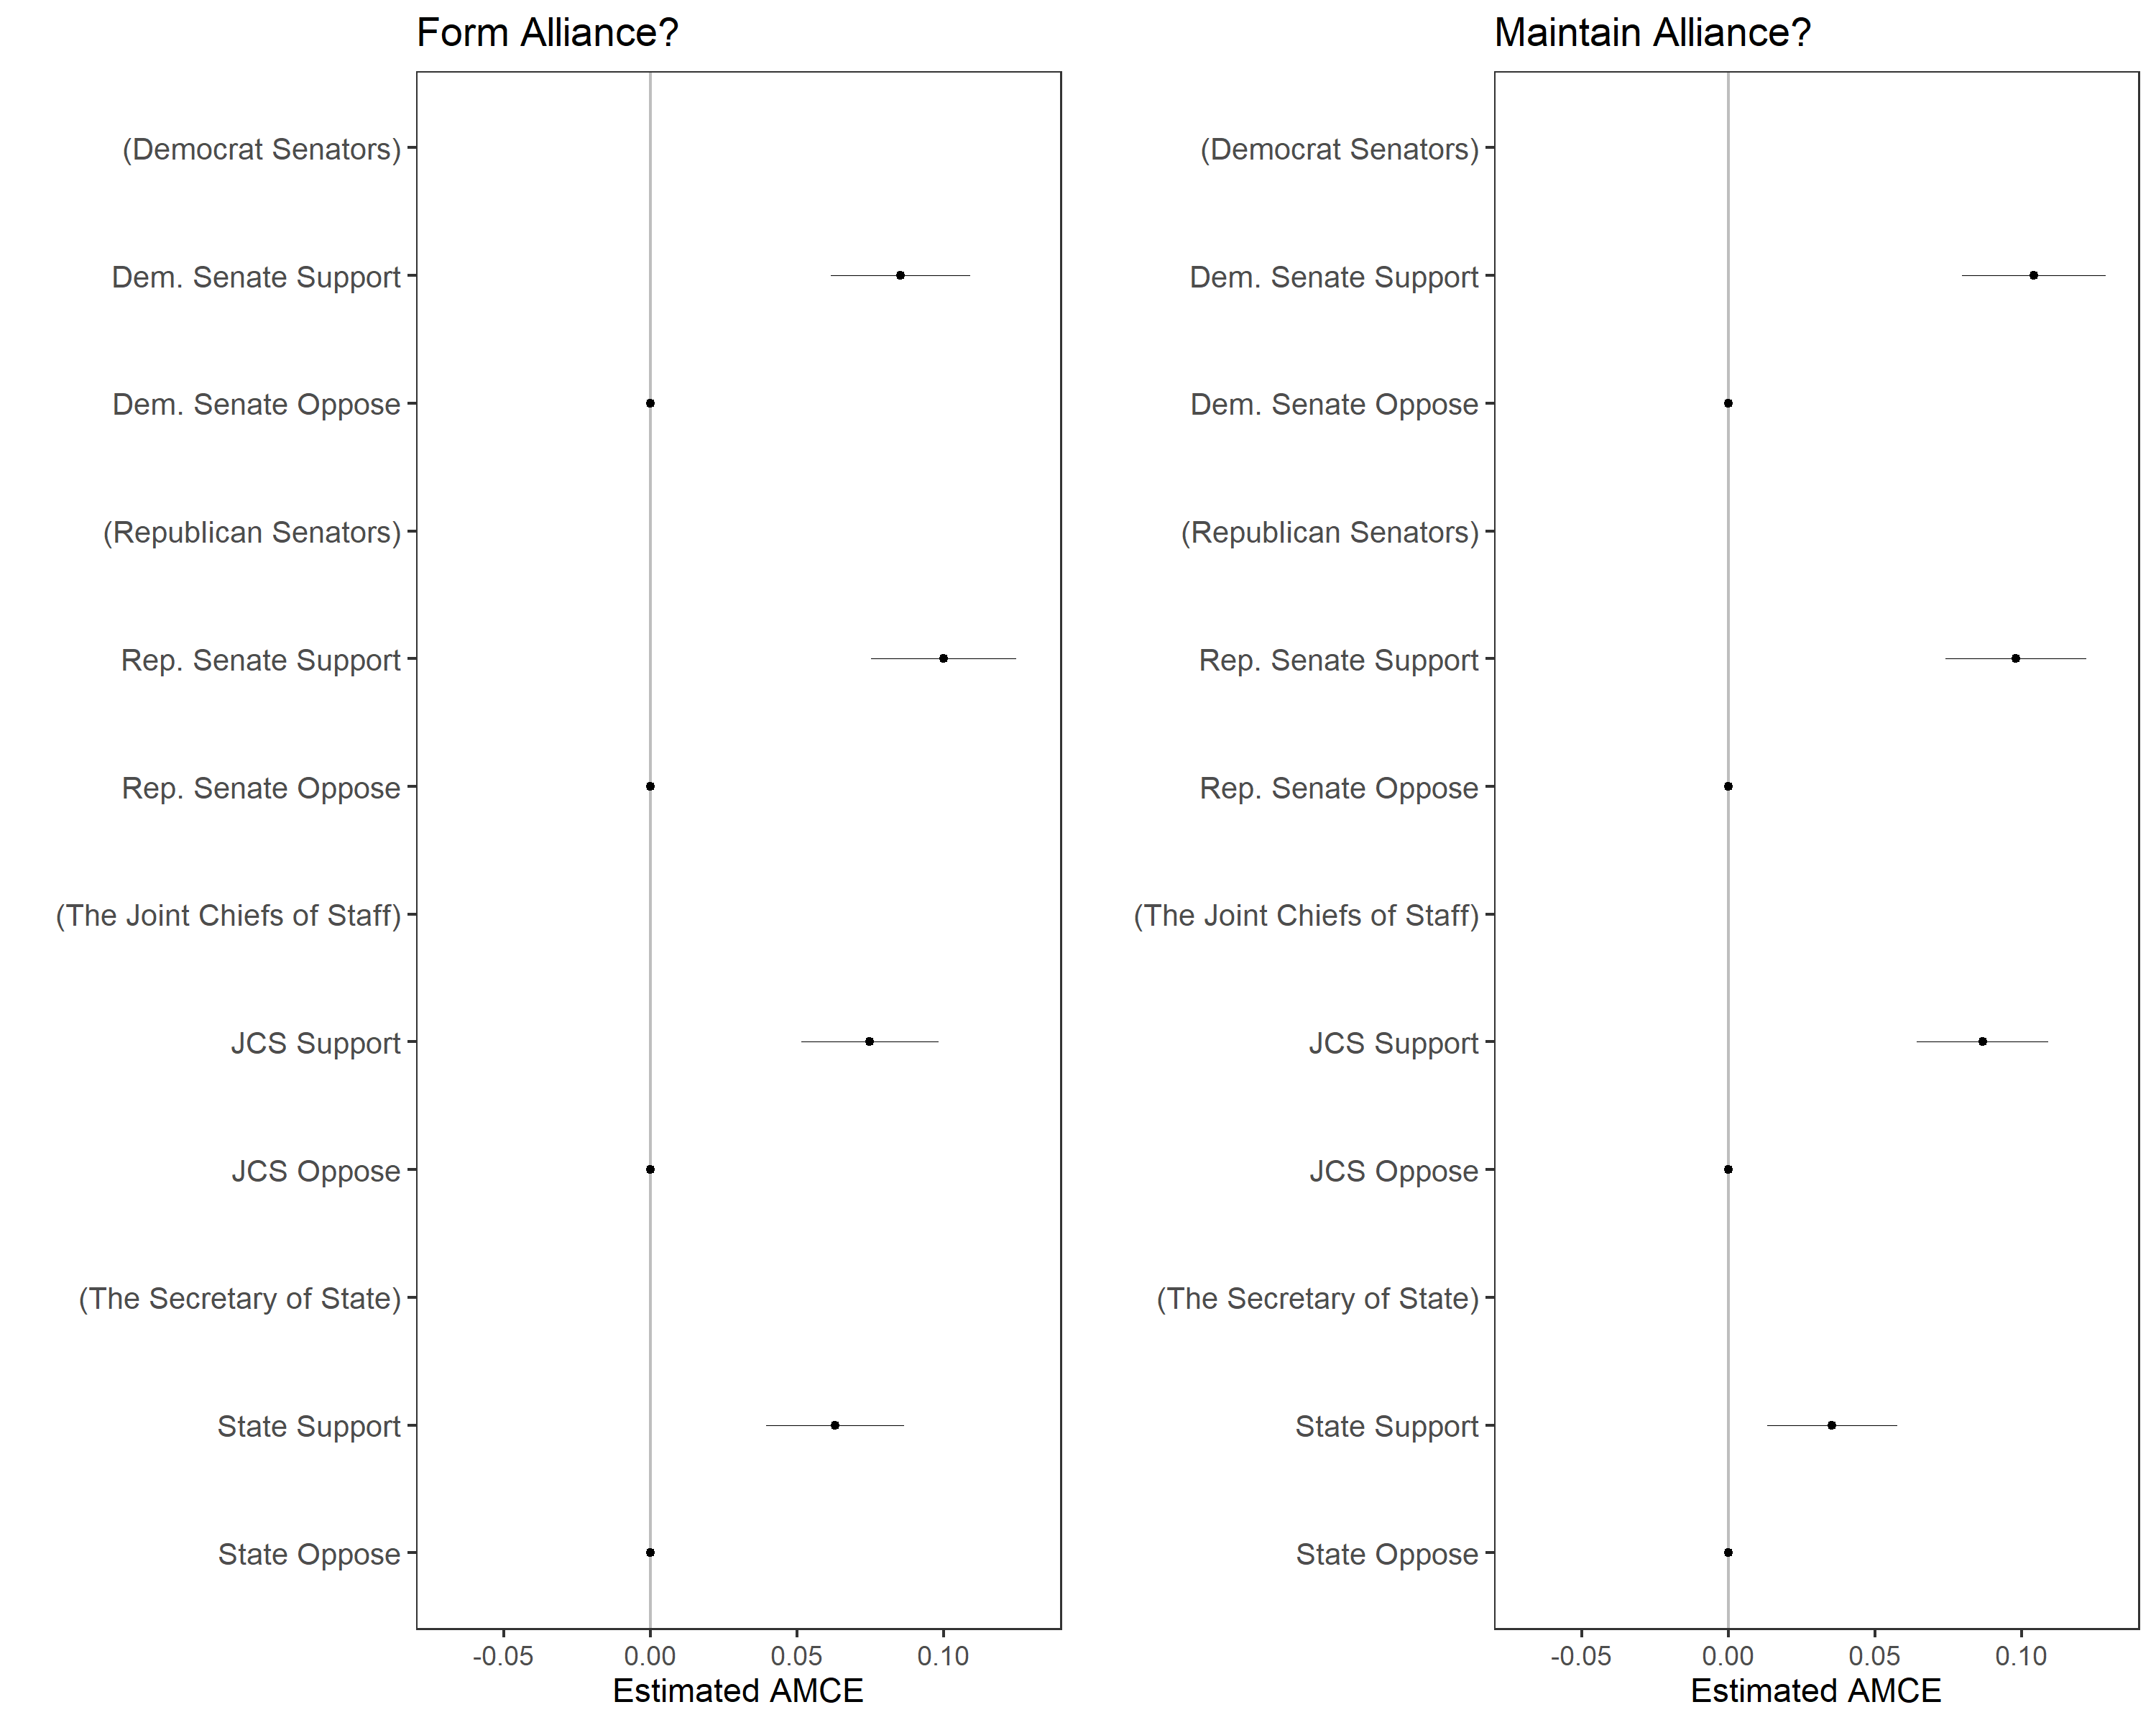
\includegraphics[width=0.95\textwidth]{../figures/joint-amce-plots-el.png}
	\caption{Average marginal component effect of elite cues on public support for forming or maintaining a hypothetical military alliance. Feature names in parentheses. Estimates with a dot at zero are the base attribute level. Components marked with abbreviated labels and all alliance characteristic attributes omitted to make the plot more legible.}
	\label{fig:joint-plot}
\end{figure}


The estimates in \autoref{fig:joint-plot} are average effects across the whole sample. 
This ignores differences in how partisanship and foreign dispositions structure foreign policy attitudes.
Examining how these factors change individual responses shows who elite cues lead.  
I therefore estimate support for alliances across respondents with different partisan affiliations and foreign policy dispositions under the expectation that extensive elite leadership implies that elite cues change attitudes regardless of foreign policy dispositions. 


\autoref{fig:party-dispo-form-el} and \autoref{fig:party-dispo-main-el} show the marginal means of support for alliance formation and maintenance from elite cues across partisan and foreign policy disposition subgroups.\footnote{The appendix summarizes the distribution of foreign policy dispositions across party identification.} 
Each panel plots the marginal mean of support for each elite cue within every categorical combination of militant assertiveness, internationalism and partisanship.
The solid vertical line in every facet marks a marginal mean of .5 and a dashed line summarizes the average alliance choice across all attributes and levels for that group.
The average choice in all experimental conditions and tasks establishes a rough baseline attitude in each group.  


There are three key findings in \autoref{fig:party-dispo-form-el} and \autoref{fig:party-dispo-main-el}. 
First, co-partisan elite cues influence most alliance attitudes, which suggests extensive elite influence. 
Second, one subgroup of each major party holds rigid alliance attitudes. 
Finally, support for alliance maintenance is more rigid than support for alliance formation. 



\begin{figure}[htpb]
	\centering
		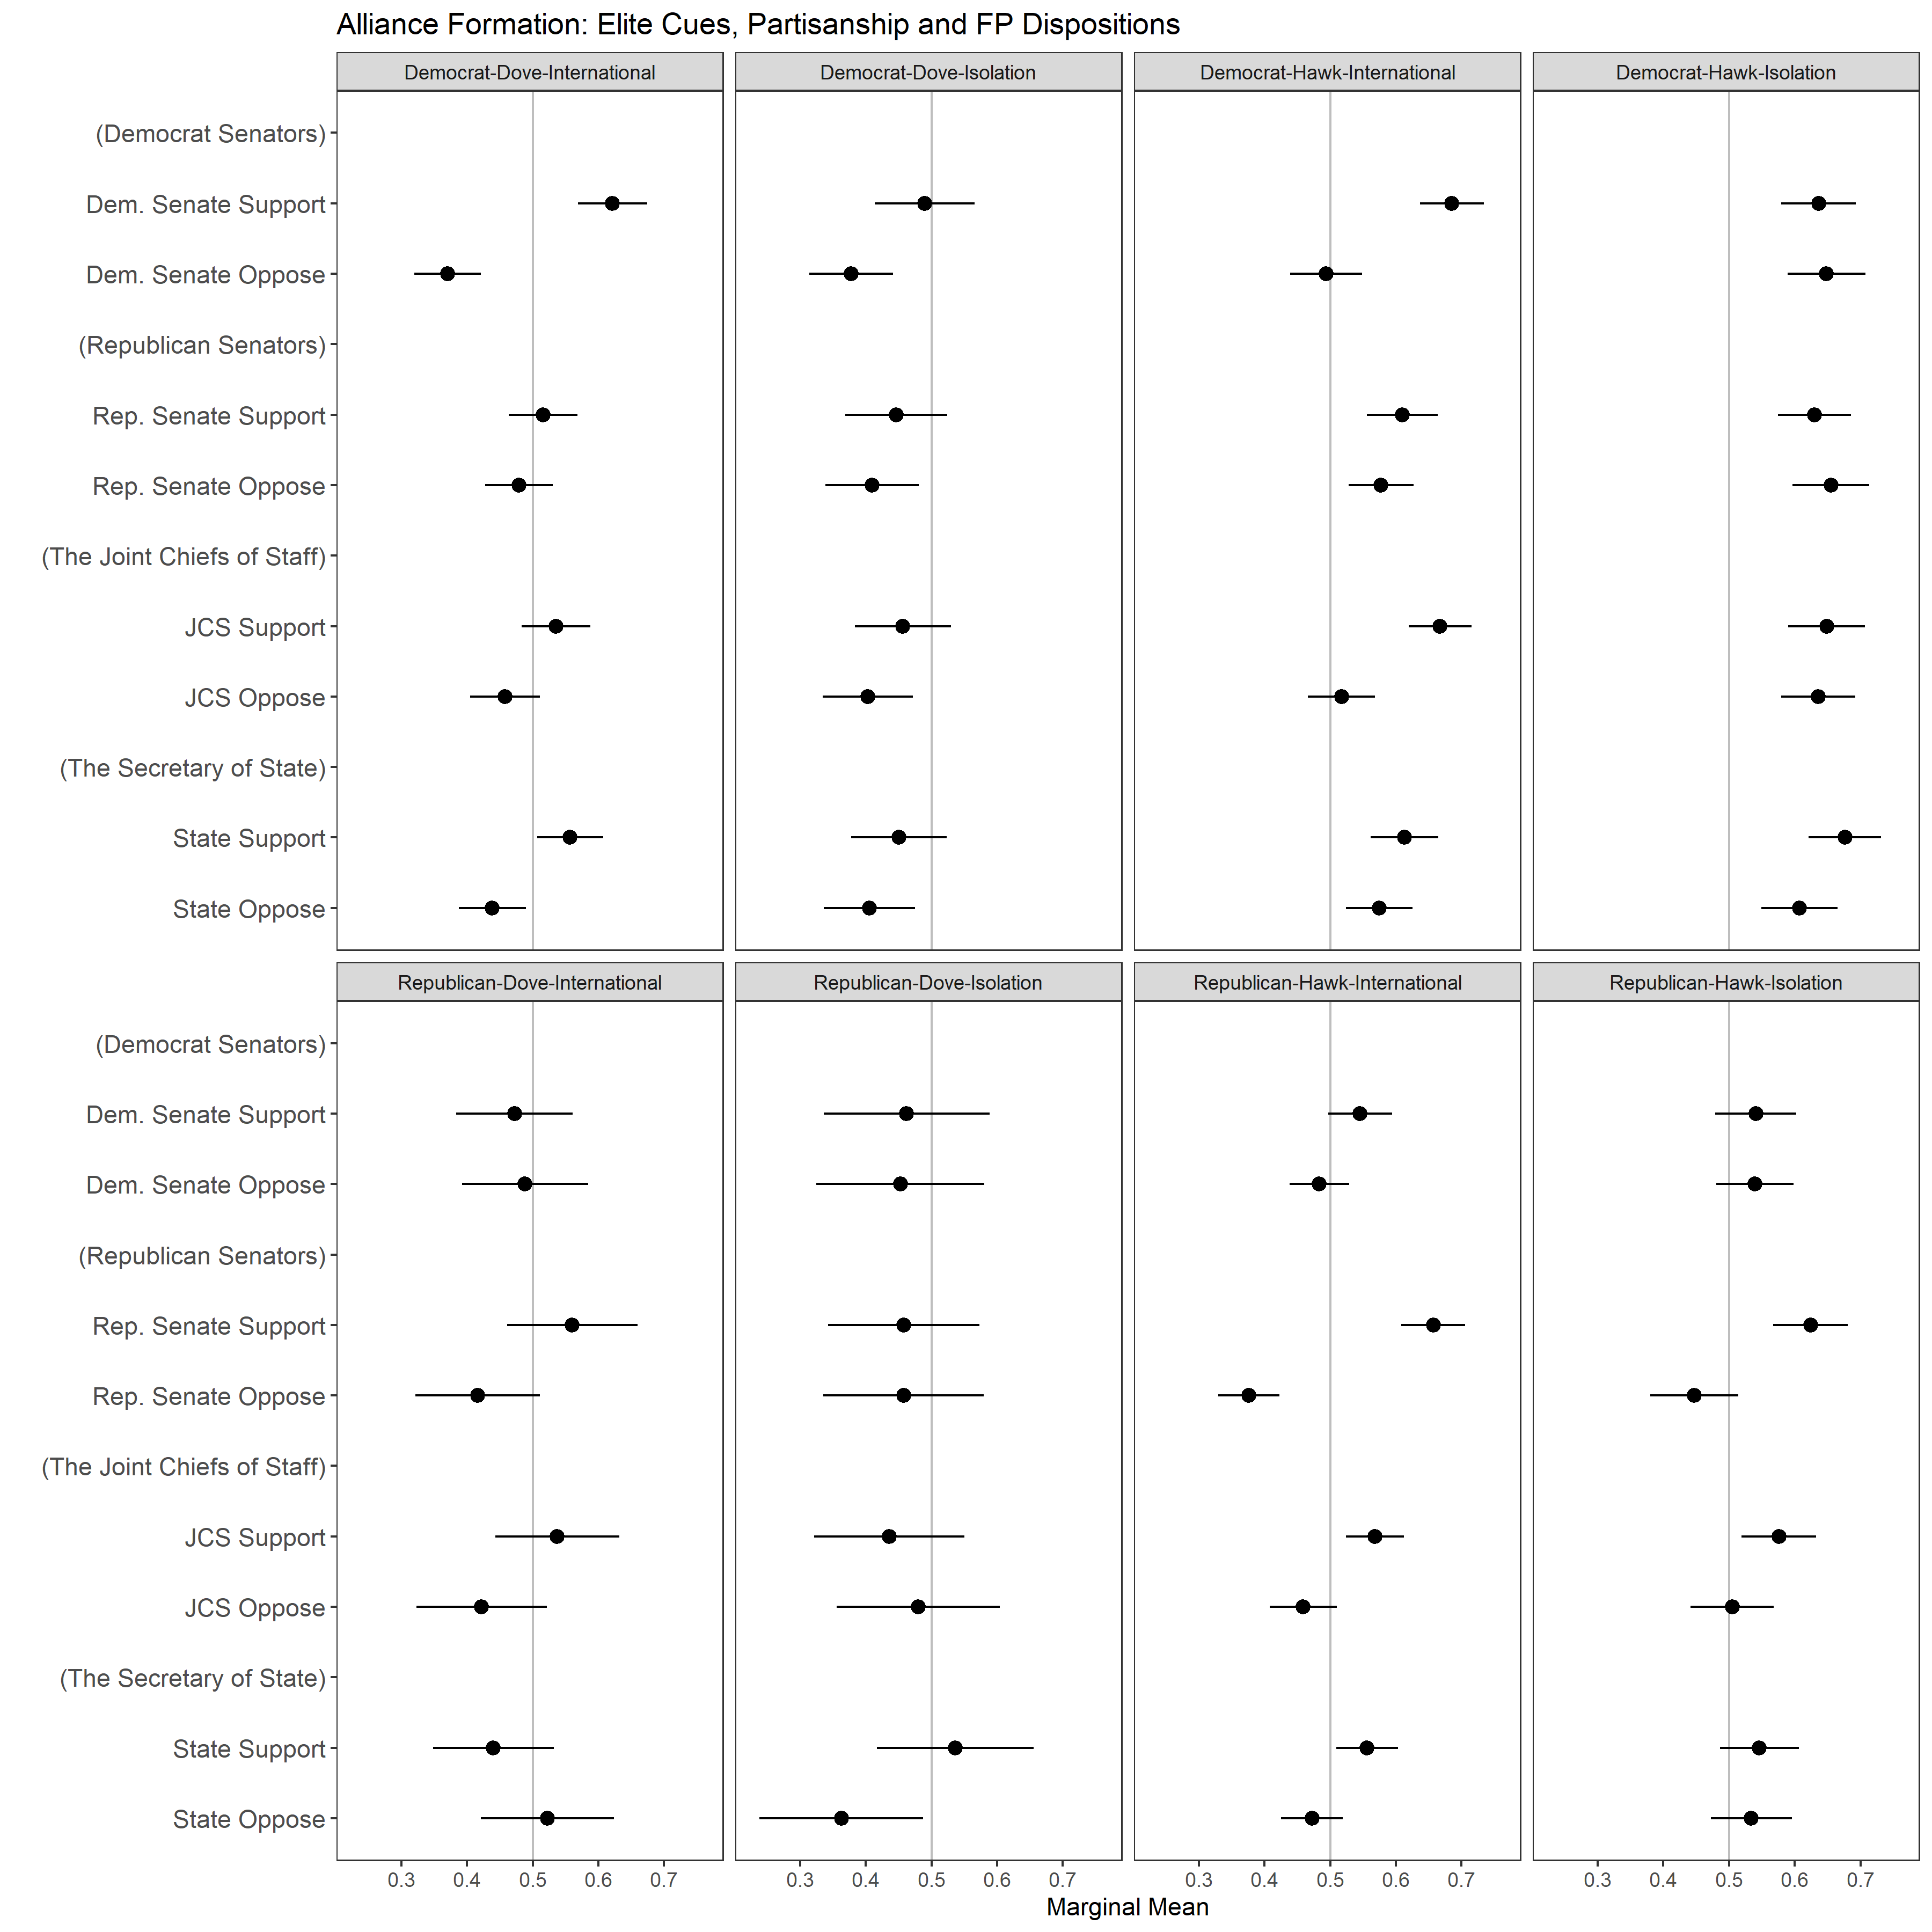
\includegraphics[width=0.95\textwidth]{../figures/party-dispo-form-el.png}
	\caption{Marginal means of support for forming hypothetical alliances across party identification and foreign policy dispositions given different elite cues. For each group, the estimates mark the marginal mean of support for alliance participation under different alliance treatments. The solid vertical line highlights a marginal mean of .5, while the dashed line marks the average choice across all levels. Components given abbreviated labels to make the plot more legible. Independents omitted.}
	\label{fig:party-dispo-form-el}
\end{figure}


Baseline alliance attitudes depend on individual concerns. 
The same foreign policy dispositions have distinct implications for alliance attitudes among Republicans and Democrats, so partisanship matters.
At the same time, foreign policy dispositions produce substantial differences in alliance attitudes within parties.  
Among Democrats and Republicans, hawkishness increases general support for alliance participation and some isolationists are less likely to heed elite cues. 
Hawkish Democrats express higher support for alliance participation than hawkish Republicans, however. 
Isolationist and hawkish Democrats are the strongest alliance participation backers. 
Hawkishness also facilitates alliance participation approval among isolationists. 


\begin{figure}
	\centering
		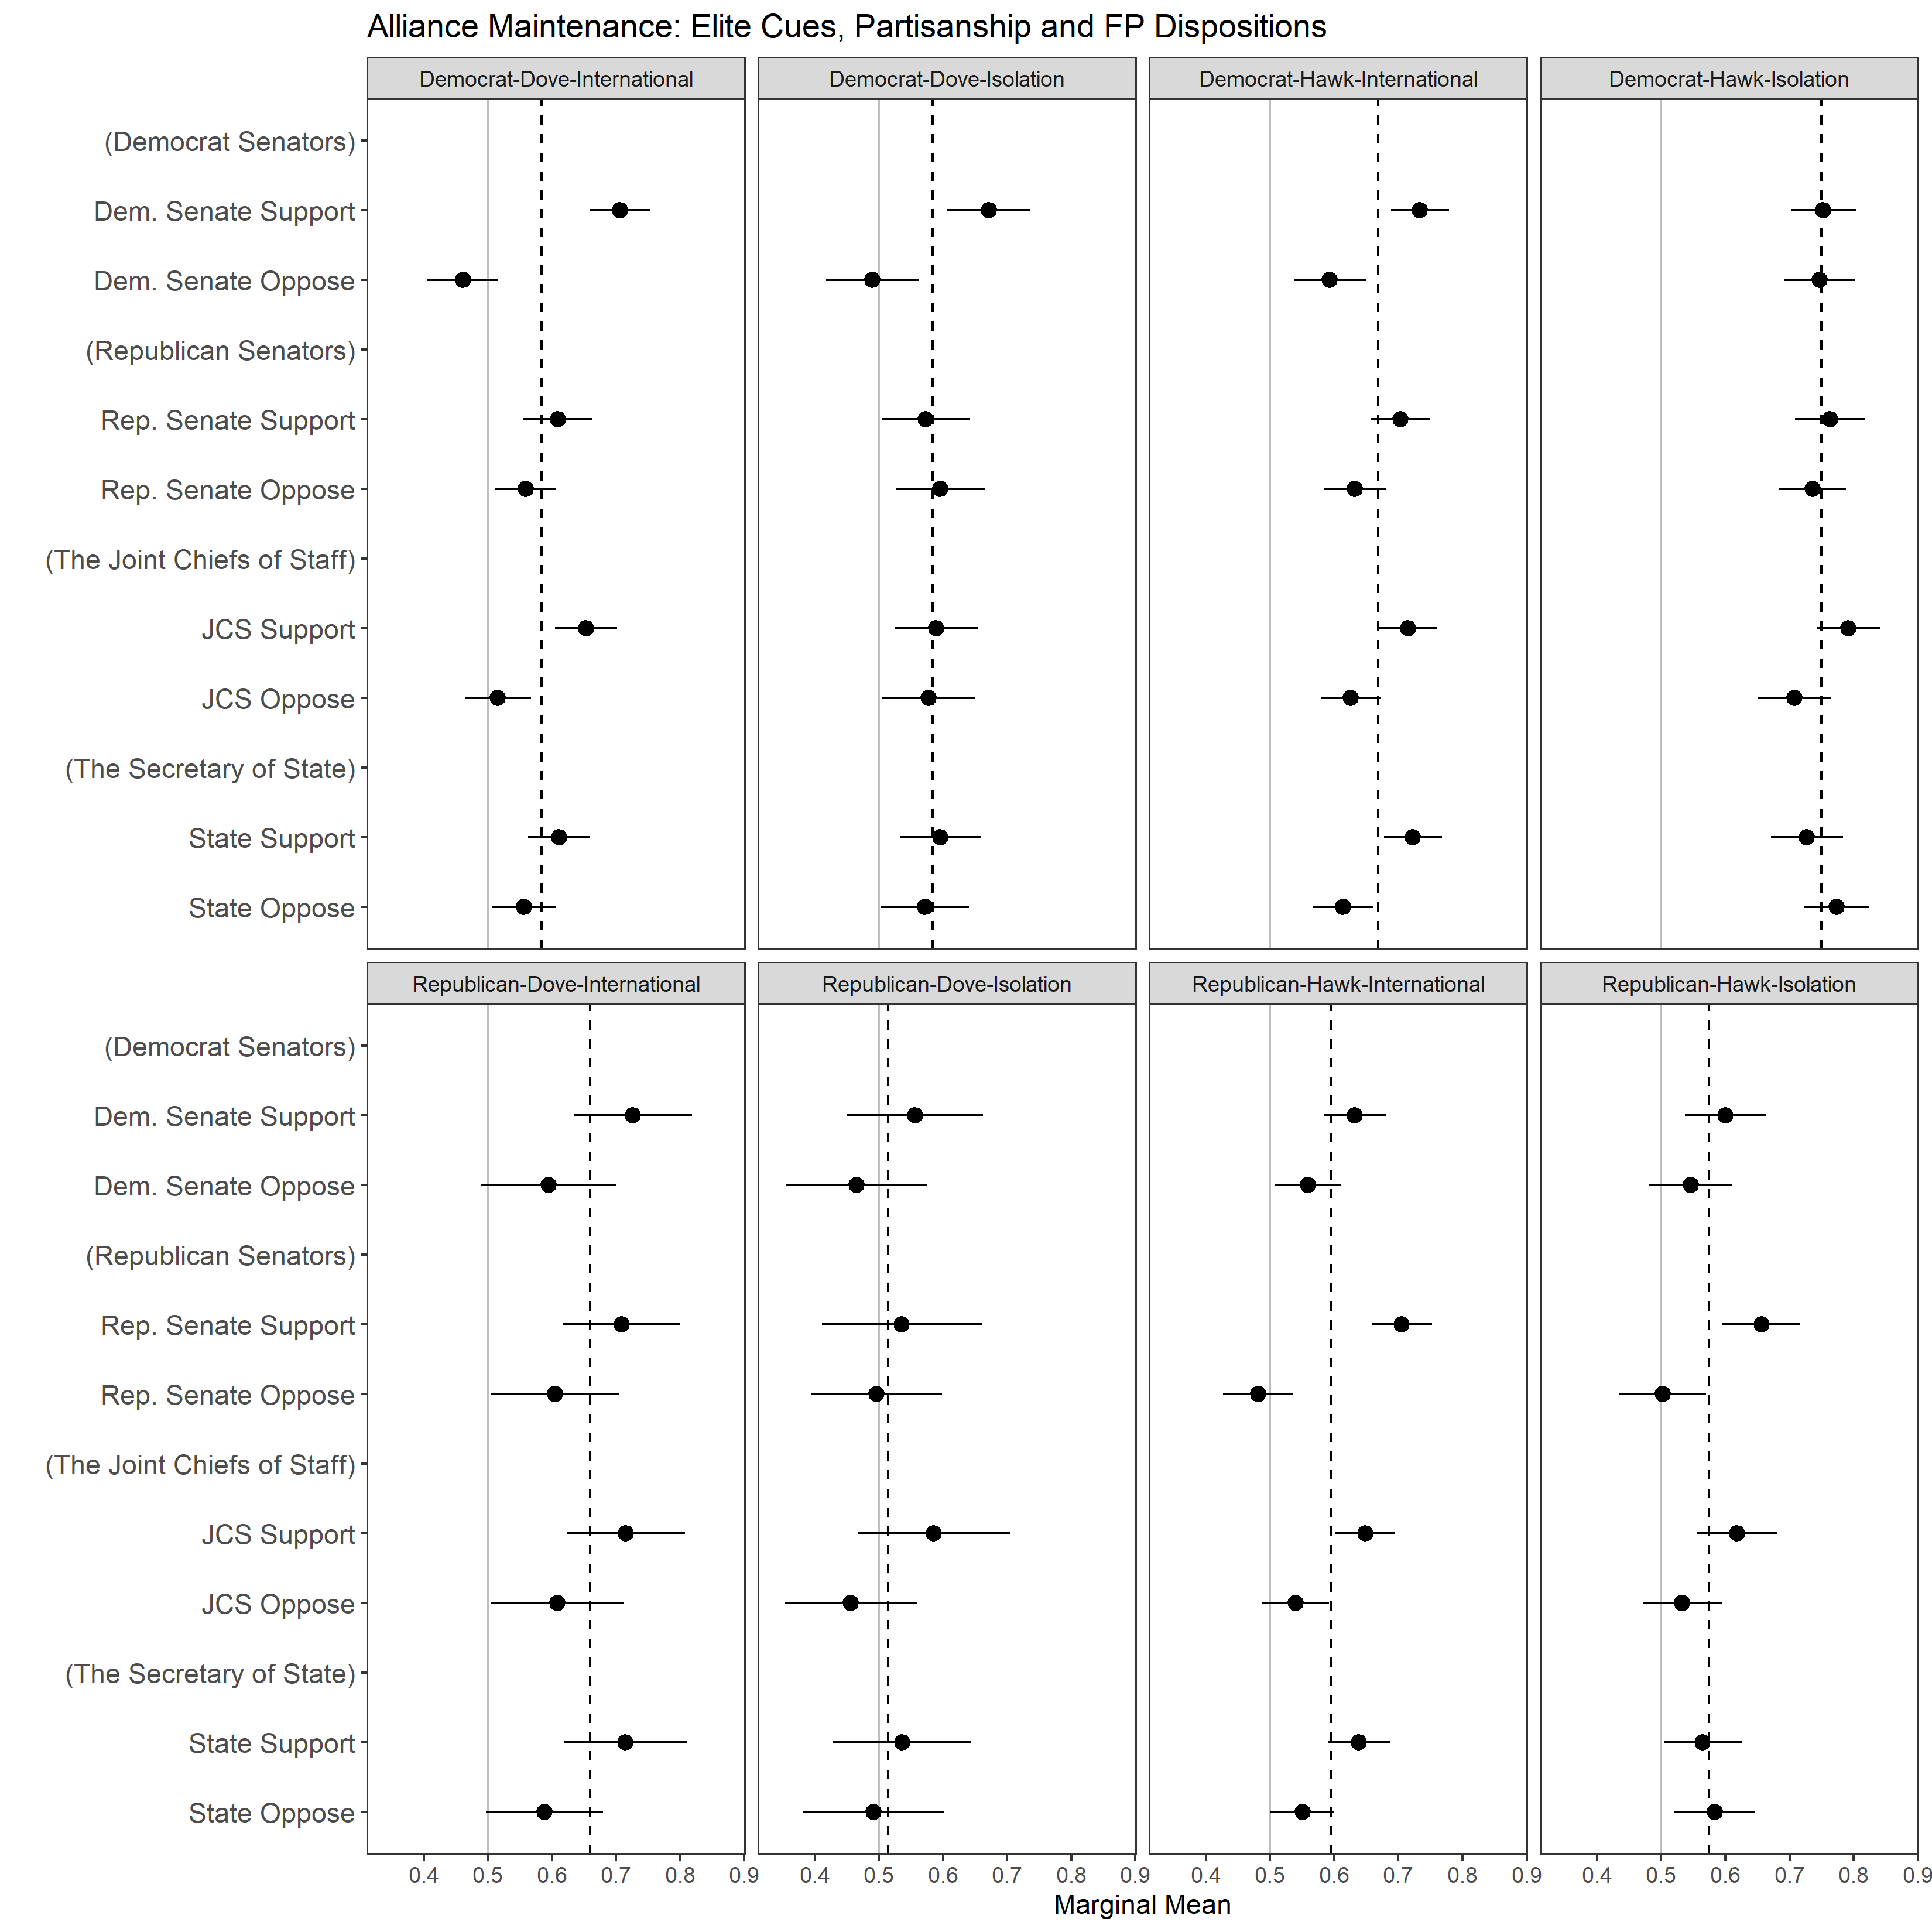
\includegraphics[width=0.95\textwidth]{../figures/party-dispo-main-el.png}
	\caption{Marginal means of support for maintaining hypothetical alliances across party identification and foreign policy dispositions given different elite cues. For each group, the estimates mark the marginal mean of support for alliance participation under different alliance treatments. The solid vertical line highlights a marginal mean of .5, while the dashed line marks the average choice across all levels. Components given abbreviated labels to make the plot more legible. Independents omitted.}
	\label{fig:party-dispo-main-el}
\end{figure}


The strongest alliance opponents are skeptics of international engagement and using military force. 
Isolationist and dovish individuals are less likely to support alliance formation and maintenance. 
Although few Republican are doves, they are integral to alliance skepticism in the GOP, especially when they also hold isolationist views.
Dovish Democrats are also more likely to oppose alliance participation.  


In addition to shifting baseline alliance attitudes, foreign policy dispositions change individual responses to elite cues. 
Internationalist Democrats respond to support from Democratic Senators, and also follow cues from the Secretary of State and Joint Chiefs of Staff. 
Hawkish and isolationist Democrats express consistent high support for forming and maintaining alliances regardless of partisan elite cues, though they may heed military elite cues on alliance maintenance. 
The strongest alliance supporters in the Democratic party thus hold rigid alliance attitudes.


Among Republicans, hawks respond to elite cues. 
Regardless of their view of international engagement, there are clear differences in alliance support for hawkish Republicans based on Republican Senate support or opposition.
Hawkish Republicans also follow cues from military elites, and internationalist hawks in the GOP further look to diplomatic leaders. 
As a result, Republican elites can lead alliance attitudes among individuals who are disposed to support forceful international engagement, so their opposition can constrain alliance support among the most likely alliance backers in their party. 
The gap in hawkish Republican attitudes from differences in Republican elite support is especially pronounced in the alliance formation experiment. 
Dovish and isolationist Republicans pay little attention to elite cues. 
The most consistent alliance opponents in the Republican party hold rigid alliance attitudes, which is the reverse of the Democratic party. 


% group size
Rigid alliance attitudes are rare. 
In the alliance formation experiment, 7\% of Republicans and 25\% of Democrats hold foreign policy dispositions that limit their response to co-partisan elite cues. 
In the alliance maintenance experiment, 9\% of Republicans and 23\% of Democrats have similarly rigid alliance attitudes.
Republicans are thus more likely to respond to elite cues.


% highlight differences in formation and maintenace
Individuals express distinct attitudes towards alliance formation and maintenance. 
Forming new alliances draws lower baseline support than maintaining existing treaties, so elite cues are crucial. 
Only hawkish Democrats express clear support for alliance formation--- other respondents are divided or oppose new treaties on average.
Dovish isolationists dislike new alliances, though elites can persuade Democrats with this disposition. 
Whether elites support or oppose an alliance determines whether it has majority or minority support within each party. 


Alliance maintenance commands more robust support than alliance formation. 
Regardless of elite cues, the overall average and marginal means of support for alliance maintenance are almost all above .5. 
Even dovish isolationists in the GOP express a split verdict on alliance maintenance on average.
Although elite cues can change public attitudes, their impact on support for existing alliances has substantive limits.


% wrap up
These results suggest that elite cues exert extensive influence on alliance attitudes, especially for new treaties.
That influence is subject some important conditions, the most salient of which is a partisan asymmetry in rigid alliance attitudes. 
Democrat leaders can lead alliance skeptics and have less influence over the most committed alliance supporters. 
Republican elites can lead alliance supporters, but do not persuade committed alliance skeptics. 
As a result, elite cues have substantial influence on most individuals in both parties, but the strongest alliance attitudes condition their impact. 


An online appendix provides further support for these results. 
In the appendix, I present conditional marginal means for key alliance characteristics, examine marginal means by partisanship and foreign policy dispositions alone, analyze responses to an open-ended question, and compare results with the continuous rating measure of alliances to inferences from the choice question.
All the checks are consistent with these findings. 


\section{Discussion and Conclusion} 


% Overview
I find extensive elite leadership of public alliance attitudes with some limits.  
Most individuals follow co-partisan elite cues, but their exact response depends on partisanship, hawkishness and isolationism, because individual concerns set baseline attitudes.
Support for alliance maintenance is less response to elite cues than support for alliance formation as well. 
Moreover, a few individuals hold rigid alliance opinions.  
The most committed alliance supporters ---hawkish and isolationist Democrats--- pay little attention to elite cues.
Similarly, elite cues have no impact on the most committed alliance skeptics; dovish and isolationist Republicans. 
Republicans can lead co-partisan alliance supporters, while Democrats can lead co-partisan alliance skeptics. 


% bring it in on observed alliances
These findings have three implications for understanding public attitudes towards U.S. alliances like NATO. 
First, the Republican and Democratic parties contain committed alliance skeptics and supporters, respectively.
In the two representative samples, roughly a quarter of Democrats are strong alliance supporters and approximately 8\% of Republicans are staunch alliance skeptics.
Outside these groups and independents, most Americans follow partisan elite cues in forming alliance attitudes. 
This makes whether elites follow fixed alliance attitudes in their party a critical issue, because it would polarize alliance attitudes in everyone else.  


Second, my findings support the view that elite-driven public opinion cycles could make democratic commitments less reliable \citep{GartzkeGleditsch2004}. 
Although the results suggest that many members of the public hold considered opinions \citep{PageShapiro1992}, they also show substantial elite influence. 
Elite opposition rarely pushes alliance attitudes into majority opposition to existing treaties, but elite cues can reduce aggregate support in both major parties.
In the Republican Party, elite opposition creates an even split in alliance maintenance attitudes. 
Negative cues from military or diplomatic elites could bolster the impact of skeptical politicians and cut public support. 


% why NATO robust under Trump? 
Finally, these results help us understand public opinion towards alliances like NATO during the Trump administration.
Although Trump often criticized U.S. allies, alliance commitments usually commanded majority support throughout his administration \citep{PewNATO2020}. 
The relative stability of alliance attitudes reflects Democrats' aversion to Trump, countervailing cues from other elites and high baseline support for existing alliances.
Hawkishness offsets the tendency of isolationism to increase alliance skepticism for many Republicans.
Although Trump likely increased Republican opposition to alliances, his influence on attitudes towards existing commitments faced meaningful constraints. 


% limitations
These findings have some limitations. 
For one, while the sheer variety of alliances means that the above profiles are plausible, extrapolating from the survey experiments to observed alliances is inexact. 
The artificial nature of a survey experiment provides essential control to disentangle public attitudes, but no hypothetical alliance can fully reflect real world commitments.
Some confounding of elite cues is possible, as the experiment cannot include every potentially relevant alliance characteristic. 
Moreover, elites have other ways to move public opinion besides direct cues, so this may be a simple first test of how elites shape alliance attitudes. 


% can't show pandering
While this paper provides new insight into elite leadership of foreign policy opinion, it does not give a comprehensive account of elite-public interactions.
It shows that elites can lead, but not when and why they choose to exercise that influence. 
How much and when elites might decide to follow fixed alliance attitudes in their party also falls outside the scope of this paper. 
Understanding the long-run dynamics of leading and following as well as when elites employ different strategies is a crucial subject for future research. 


% non-us results- might be different, subject for future inquiry
Furthermore, this study focuses on the United States, which has an unusual alliance network. 
Though public opinion towards alliances in the United States is important, attitudes in other countries matter as well. 
Future research should examine the sources of alliance attitudes in other countries. 


% future stuff: feedback, content of elite cues
These results provide a foundation for further inquiry into the domestic politics of military alliances. 
Two questions are especially interesting in this respect.
First, how much feedback takes place between public opinion and elite cues? 
When do politicians follow rigid alliance attitudes or lead in a competing direction? 
Politicians might view marginal opinion shifts due to threat or allied democracy changes as an opportunity to encourage or arrest further changes in public support.
Second, would leaders face significant public disapproval if they withdrew from an alliance? 
This study focused on generic support, but future research should build on \citet{TomzWeeks2021} and examine specific alliance policy changes. 


These questions address how elites form and maintain domestic coalitions around international engagement. 
In the 75 years since the end of World War II, shifting elite cues, partisanship, generational experiences and allied characteristics may mean different groups back alliances today than in 1950. 
Tracking changes in the domestic coalitions backing alliances is another worthwhile task for future research.


% wrap it up 
In conclusion, elite cues exert extensive influence on alliance attitudes, subject to some important limits.
Most individuals heed elite cues, but subsets of both major parties hold rigid alliance attitudes. 
Partisan differences in elite cues and rigid alliance attitudes will thus play an important role in the future of alliance politics.



\newpage

% Bibliography
 
\bibliography{../../MasterBibliography} 




\end{document}
